\chapter{System Description}
The system comprises a ball placed on a beam that is tilted at an angle $\theta$.
The beam possesses a length $l$ and is capable of rotating around a defined pivot point.
The position of the ball on the beam is denoted by $p$, where $x = 0$ corresponds to the left end of the beam,
and $p = l$ corresponds to the right end.
The beam connects to a motor via a gear mechanism, where the distance from the motor's rotor to the gear arm is represented as $d$. The gear arrangement enables the motor to apply a torque $\tau$ to the beam, inducing its rotation about the pivot point.
Additionally, the system involves the parameter $\phi$, which signifies the gear angle.
This angle $\phi$ characterizes the orientation of the gear linked to the motor. As the motor rotates,
the gear angle $\phi$ changes, influencing the torque exerted on the beam and consequently impacting its position and tilt angle $\theta$.
The motion of the ball and the rotation of the beam are intricately linked through factors such as the motor's torque,
the gear angle $\phi$, and the distance $d$ from the rotor to the gear arm.
The system's dynamic behavior is governed by these interrelated variables,
leading to diverse motion patterns and equilibrium conditions for the ball on the tilted beam.
The comprehension and analysis of this system entail investigating the relationships among variables $l$, $x$, $d$, $\theta$, and $\phi$, as well as considering the influence of external forces like gravity and potential control inputs.
Utilizing mathematical models and principles from mechanics enables the characterization and prediction of the system's behavior across various scenarios.
% Symbols
\nomenclature{$l$}{Length of the beam}
\nomenclature{$p$}{Position of the ball on the beam}
\nomenclature{$d$}{Distance from the motor's rotor to the gear arm}
\nomenclature{$\phi$}{Gear angle}
\nomenclature{$\theta$}{Tilt angle of the beam}
\nomenclature{$r$}{Ball's radius}
\nomenclature{$\tau$}{External torque applied to the beam}
\begin{figure}[ht]
	\centering
	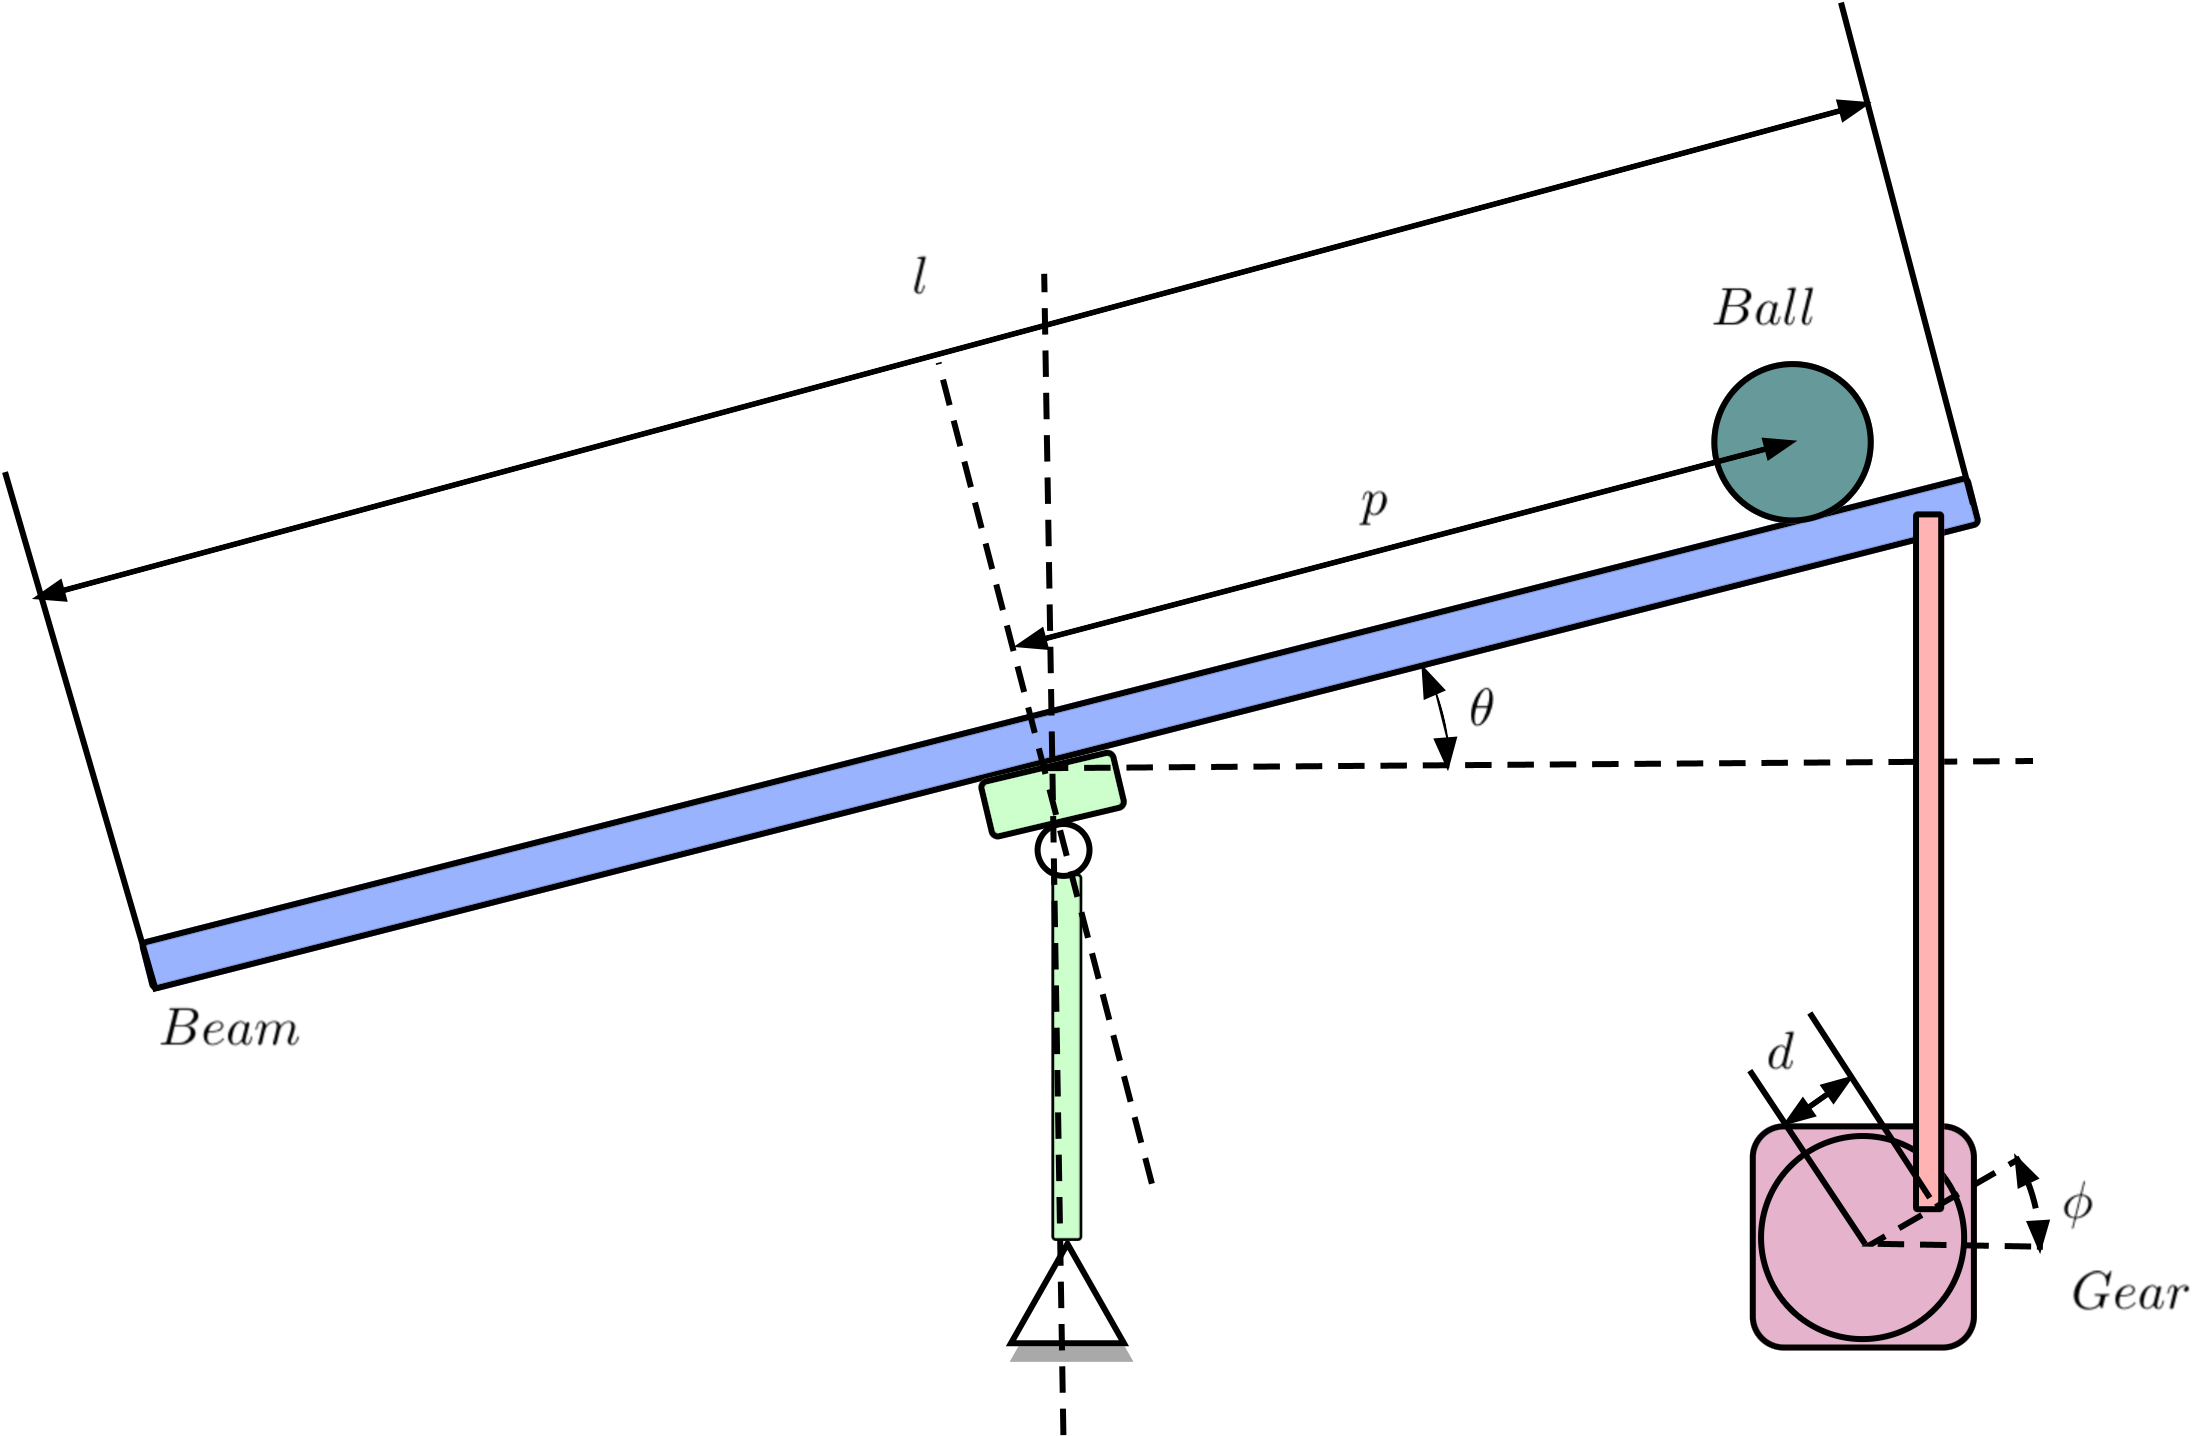
\includegraphics[height =7.5cm,width =10cm]{System_Overview}
	\caption{System Overview}
\end{figure}
